Sed ut perspiciatis unde omnis iste natus error sit voluptatem accusantium doloremque laudantium.

With a different Footnote\footnote{Another footnote}, bold text \textbf{emphasized text} and a citation~\cite{einstein2013principle}. Let's add some math $y = mx + c$ and italics \textit{highlighted}. And also itemize and lists:
\begin{itemize}
	\item Item A
	\item Item B
\end{itemize}
\begin{enumerate}
	\item Item Alpha
	\item Item Beta
\end{enumerate}
And some figures:
\begin{figure}[H]
	\centering
	% but image scaling doesn't work!!
	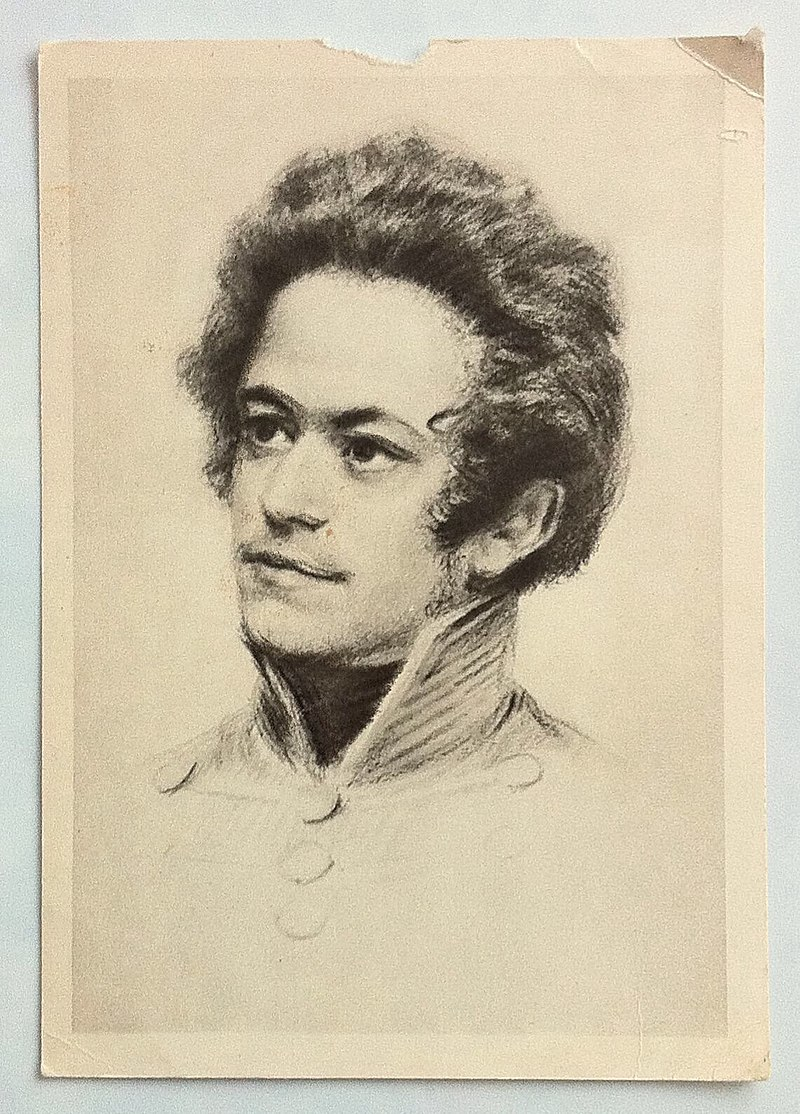
\includegraphics[scale=0.5]{../resources/sample-image.png}
	\caption{A sample image}
	\label{fig:sample}
\end{figure}

And tables:
\begin{table}[H]
	\centering
	\begin{tabular}{|c|c|}
		\hline
		C & D \\ \hline
		3 & 4 \\ \hline
	\end{tabular}
	\caption{A sample table}
	\label{tab:sample}
\end{table}

And you can reference them: a figure~\ref{fig:sample}, a table~\ref{tab:sample}.

% bibliography can be added
\bibliography{../resources/Bibliography}
